%%%%%%%%%%%%%%%%%%%%%%%%%%%%%%%%%%%%%%%%%
% Masters/Doctoral Thesis 
% LaTeX Template
% Version 2.5 (27/8/17)
%
% This template was downloaded from:
% http://www.LaTeXTemplates.com
%
% Version 2.x major modifications by:
% Vel (vel@latextemplates.com)
%
% This template is based on a template by:
% Steve Gunn (http://users.ecs.soton.ac.uk/srg/softwaretools/document/templates/)
% Sunil Patel (http://www.sunilpatel.co.uk/thesis-template/)
%
% Template license:
% CC BY-NC-SA 3.0 (http://creativecommons.org/licenses/by-nc-sa/3.0/)
%
%%%%%%%%%%%%%%%%%%%%%%%%%%%%%%%%%%%%%%%%%

%----------------------------------------------------------------------------------------
%	PACKAGES AND OTHER DOCUMENT CONFIGURATIONS
%----------------------------------------------------------------------------------------

\PassOptionsToPackage{greek,main=english}{babel}

\documentclass[
11pt, % The default document font size, options: 10pt, 11pt, 12pt
%oneside, % Two side (alternating margins) for binding by default, uncomment to switch to one side
english, % ngerman for German
onehalfspacing, % Single line spacing, alternatives: onehalfspacing or doublespacing
%draft, % Uncomment to enable draft mode (no pictures, no links, overfull hboxes indicated)
%nolistspacing, % If the document is onehalfspacing or doublespacing, uncomment this to set spacing in lists to single
%liststotoc, % Uncomment to add the list of figures/tables/etc to the table of contents
%toctotoc, % Uncomment to add the main table of contents to the table of contents
parskip, % Uncomment to add space between paragraphs
%nohyperref, % Uncomment to not load the hyperref package
headsepline, % Uncomment to get a line under the header
%chapterinoneline, % Uncomment to place the chapter title next to the number on one line
%consistentlayout, % Uncomment to change the layout of the declaration, abstract and acknowledgements pages to match the default layout
]{MastersDoctoralThesis} % The class file specifying the document structure

\let\thesisdegree=\degree
\undef\degree

\usepackage[T1]{fontenc} % Output font encoding for international characters
\usepackage[utf8]{inputenc} % Required for inputting international characters

\usepackage{mathpazo} % Use the Palatino font by default
\usepackage{comment}
\usepackage{lscape}
\usepackage{minted}
\usemintedstyle{friendly}
\usepackage{xcolor}
\definecolor{light-gray}{gray}{0.95}
\usepackage{amsmath}
\usepackage{gensymb}
\setlength\parindent{0pt}
\usepackage{microtype}
\usepackage{hyperref}
\usepackage[nameinlink,capitalise]{cleveref}
\usepackage{siunitx}


\usepackage[backend=bibtex,style=numeric,natbib=true,sorting=none]{biblatex} % Use the bibtex backend with the authoryear citation style (which resembles APA)

\addbibresource{bibliography.bib} % The filename of the bibliography

\usepackage[autostyle=true]{csquotes} % Required to generate language-dependent quotes in the bibliography

%----------------------------------------------------------------------------------------
%	MARGIN SETTINGS
%----------------------------------------------------------------------------------------

\geometry{
	paper=a4paper, % Change to letterpaper for US letter
	inner=2.5cm, % Inner margin
	outer=3.8cm, % Outer margin
	bindingoffset=.5cm, % Binding offset
	top=1.5cm, % Top margin
	bottom=1.5cm, % Bottom margin
	%showframe, % Uncomment to show how the type block is set on the page
}

%----------------------------------------------------------------------------------------
%	THESIS INFORMATION
%----------------------------------------------------------------------------------------

\thesistitle{Image based orbit determination of the Didymos-Dimorphos binary asteroid system using the HERA spacecraft} % Your thesis title, this is used in the title and abstract, print it elsewhere with \ttitle
\supervisor{Prof. Kleomenis \textsc{Tsiganis}} % Your supervisor's name, this is used in the title page, print it elsewhere with \supname
\examiner{} % Your examiner's name, this is not currently used anywhere in the template, print it elsewhere with \examname
\thesisdegree{Computational Physics} % Your degree name, this is used in the title page and abstract, print it elsewhere with \degreename
\author{Anastasios-Faidon \textsc{Retselis}} % Your name, this is used in the title page and abstract, print it elsewhere with \authorname
\addresses{} % Your address, this is not currently used anywhere in the template, print it elsewhere with \addressname

\subject{Physics} % Your subject area, this is not currently used anywhere in the template, print it elsewhere with \subjectname
\keywords{} % Keywords for your thesis, this is not currently used anywhere in the template, print it elsewhere with \keywordnames
\university{\href{http://www.auth.gr}{Aristotle University of Thessaloniki}} % Your university's name and URL, this is used in the title page and abstract, print it elsewhere with \univname
\department{\href{https://www.physics.auth.gr/}{Physics Department}} % Your department's name and URL, this is used in the title page and abstract, print it elsewhere with \deptname
\group{\href{http://acubesat.asat.gr}{AcubeSAT Project}} % Your research group's name and URL, this is used in the title page, print it elsewhere with \groupname
\faculty{\href{http://www.sci.auth.gr}{Faculty of Sciences}} % Your faculty's name and URL, this is used in the title page and abstract, print it elsewhere with \facname

\AtBeginDocument{
\hypersetup{pdftitle=\ttitle} % Set the PDF's title to your title
\hypersetup{pdfauthor=\authorname} % Set the PDF's author to your name
\hypersetup{pdfkeywords=\keywordnames} % Set the PDF's keywords to your keywords
\hypersetup{bookmarksnumbered=true} % Add numbering to PDF bookmarks
}

\begin{document}
\hypersetup{urlcolor=blue}
\hypersetup{linkcolor=blue}
\hypersetup{citecolor=cyan}
\frontmatter % Use roman page numbering style (i, ii, iii, iv...) for the pre-content pages


\pagestyle{plain} % Default to the plain heading style until the thesis style is called for the body content

%----------------------------------------------------------------------------------------
%	TITLE PAGE
%----------------------------------------------------------------------------------------

\begin{titlepage}
\begin{center}

\begin{figure}[H]
\centering

\includegraphics[scale=0.4]{Figures/LogoAUTH72ppi.png}
%\label{fig:auth_logo}
\end{figure}

\vspace*{.04\textheight}
{\scshape\LARGE \univname\par}\vspace{1cm} % University name
\textsc{\Large Master Thesis}\\[0.5cm] % Thesis type

\HRule \\[0.4cm] % Horizontal line
{\huge \bfseries \ttitle\par}\vspace{0.4cm} % Thesis title
\HRule \\[1cm] % Horizontal line
 
\begin{minipage}[t]{0.4\textwidth}
\begin{flushleft} \large
\emph{Author:}\\
\href{https://gitlab.com/retse}{Anastasios-Faidon \textsc{Retselis}}
\end{flushleft}
\end{minipage}
\begin{minipage}[t]{0.4\textwidth}
\begin{flushright} \large
\emph{Supervisor:} \\
\href{http://users.auth.gr/tsiganis/}{Prof. Kleomenis \textsc{Tsiganis}}
\end{flushright}
\end{minipage}\\[1cm]
 
\vfill

\large \textit{A thesis submitted in fulfillment of the requirements\\ for the Master of Science (MSc) in \degreename}\\[0.3cm] % University requirement text
\textit{in the}\\[0.4cm]
\facname\\\deptname\\[1cm] % Research group name and department name
 
\vfill

{\large \today}\\[4cm] % Date
%\includegraphics{Logo} % University/department logo - uncomment to place it
 
\vfill
\end{center}
\end{titlepage}

%----------------------------------------------------------------------------------------
%	DECLARATION PAGE
%----------------------------------------------------------------------------------------

%\begin{declaration}
%\addchaptertocentry{\authorshipname} % Add the declaration to the table of contents
%\noindent I, \authorname, declare that this thesis titled, \enquote{\ttitle} and the work presented in it are my own. I confirm that:

%\begin{itemize} 
%\item This work was done wholly or mainly while in candidature for a research degree at this University.
%\item Where any part of this thesis has previously been submitted for a degree or any other qualification at this University or any other institution, this has been clearly stated.
%\item Where I have consulted the published work of others, this is always clearly attributed.
%\item Where I have quoted from the work of others, the source is always given. With the exception of such quotations, this thesis is entirely my own work.
%\item I have acknowledged all main sources of help.
%\item Where the thesis is based on work done by myself jointly with others, I have made clear exactly what was done by others and what I have contributed myself.\\
%\end{itemize}
 
%\noindent Signed:\\
%\rule[0.5em]{25em}{0.5pt} % This prints a line for the signature
 
%\noindent Date:\\
%\rule[0.5em]{25em}{0.5pt} % This prints a line to write the date
%\end{declaration}

%cleardoublepage
\cleardoublepage

%----------------------------------------------------------------------------------------
%	QUOTATION PAGE
%----------------------------------------------------------------------------------------

%\vspace*{0.2\textheight}

%\noindent\enquote{\itshape Thanks to my solid academic training, today I can write hundreds of words on virtually any topic without possessing a shred of information, which is how I got a good job in journalism.}\bigbreak

%\hfill Dave Barry

%----------------------------------------------------------------------------------------
%	ABSTRACT PAGE
%----------------------------------------------------------------------------------------

\begin{abstract}{\byname{}\authorname}
\addchaptertocentry{\abstractname} % Add the abstract to the table of contents
The number of small- and nano-satellites being launched into orbit is expected to continue to grow in the coming years. In order to avoid the creation of space debris, spacecraft developers have to take action in order to reduce the severity of space debris. A widely used guideline is to ensure that no space system is left in the Low Earth Orbit environment for more than 25 years after the end of mission. Given this guideline, this thesis investigates 1U, 2U and 3U CubeSats in Low Earth Orbit using the General Mission Analysis Tool (GMAT) in order to determine the maximum allowable value of the semi-major axis so that the 25 year limit is met. This analysis results in orbital decay diagrams which can be used by CubeSat developers in order to evaluate different orbits early in the design phase.

These findings are then applied to the AcubeSAT mission in order to perform an orbital analysis tailored to the mission. AcubeSAT is a 3U CubeSat that is currently being designed by students in the Aristotle University of Thessaloniki with the support of the Education Office of the European Space Agency, under the educational Fly Your Satellite! Programme. The objective of AcubeSAT's mission is to probe the expression of eukaryotic genes in the environment of Low Earth Orbit. AcubeSAT's design calls for a very specific orientation to be achieved in order to downlink all images to the ground segment. This orientation is evaluated using the theory of spin-orbit coupling to determine if this orientation can be maintained in the event of a failure in the Attitude Determination \& Control Subsystem of the spacecraft. Based on the findings, an alternative design solution is also proposed.

\end{abstract}

{
    \makeatletter
    \def\facname{\foreignlanguage{greek}{\href{www.sci.auth.gr}{Σχολή Θετικών Επιστημών}}}
    \def\deptname{\foreignlanguage{greek}{\href{www.physics.auth.gr}{Τμήμα Φυσικής}}}
    \def\univname{\foreignlanguage{greek}{\href{www.auth.gr}{Αριστοτέλειο Πανεπιστήμιο Θεσσαλονίκης}}}
    \def\abstractname{\foreignlanguage{greek}{Περίληψη}}
    \def\@title{\foreignlanguage{greek}{Μελέτη τροχιάς και το πρόβλημα σύζευξης σπιν-τροχιάς για την αποστολή} AcubeSAT}
    \fontfamily{artemisia}\selectfont
    
    \begin{abstract}{\foreignlanguage{greek}{Ασημάκης \textsc{Ανθοπουλος} και Αναστάσιος-Φαίδων \textsc{Ρετσελης}}}
    \addchaptertocentry{{\fontfamily{artemisia}\selectfont\abstractname}} % Add the abstract to the table of contents
    \foreignlanguage{greek}{Ο αριθμός μικρο- και νανοδορυφόρων που πρόκειται να εκτοξευθούν σε τροχιά αναμένεται να αυξηθεί στα επόμενα χρόνια. Για να αποφευχθεί η δημιουργία διαστημικών σκουπιδιών, οι κατασκευαστές των διαστημικών σκαφών θα πρέπει να προβούν στις κατάλληλες πράξεις για να μειώσουν τον κίνδυνο των διαστημικών σκουπιδιών. Για το σκοπό αυτό χρησιμοποιείται ευρύτατα η οδηγία που αναφέρει πως κανένα διαστημικό σύστημα δεν πρέπει να μείνει στο περιβάλλον χαμηλής γήινης τροχιάς} (LEO) \foreignlanguage{greek}{για χρονικό διάστημα μεγαλύτερο των 25 ετών μετά το πέρας της αποστολής. Η εργασία αυτή ερευνά την συγκεκριμένη οδηγία για την περίπτωση των} 1U, 2U \foreignlanguage{greek}{και} 3U CubeSats \foreignlanguage{greek}{στο περιβάλλον της χαμηλής γήινης τροχιάς χρησιμοποιώντας το εργαλείο} General Mission Analysis Tool (GMAT)\foreignlanguage{greek}{, ούτως ώστε να βρεθούν τα ανώτατα όρια του μεγάλου ημιάξονα για να βρίσκεται η τροχιά κάτω από το όριο των 25 ετών}. \foreignlanguage{greek}{Η ανάλυση έχει ως αποτέλεσμα διαγράμματα που δείχνουν το χρόνο ζωής σε τροχιά συναρτήσει του αρχικού υψομέτρου, τα οποία μπορούν να χρησιμοποιηθούν από κατασκευαστές} CubeSat \foreignlanguage{greek}{σε αρχικά στάδια σχεδιασμού για να μελετηθούν διαφορετικές τροχιές.}
    
    \foreignlanguage{greek}{Τα αποτελέσματα αυτά χρησιμοποιούνται για την μελέτη της τροχιάς της αποστολής} AcubeSAT. \foreignlanguage{greek}{Το} AcubeSAT \foreignlanguage{greek}{είναι ένα} 3U CubeSAT \foreignlanguage{greek}{το οποίο σχεδιάζεται από φοιτητές του Αριστοτέλειου Πανεπιστημίου Θεσσαλονίκης με την υποστήριξη του εκπαιδευτικού γραφείου του Ευρωπαϊκού Οργανισμού Διαστήματος, υπό την αιγίδα του προγράμματος} Fly Your Satellite!. \foreignlanguage{greek}{H αποστολή} AcubeSAT \foreignlanguage{greek}{έχει ως στόχο να μελετήσει τη γονιδιακή έκφραση ευκαρυωτικών κυττάρων στο περιβάλλον της χαμηλής γήινης τροχιάς. Ο σχεδιασμός του} AcubeSAT \foreignlanguage{greek}{χρησιμοποιεί έναν συγκεκριμένο προσανατολισμό για να μπορέσει να στείλει τις εικόνες του πειράματος πίσω στη Γη. Ο προσανατολισμός αυτός διερευνάται με τη χρήση του προβλήματος σπιν-τροχιάς για να διευκρινιστεί εαν μπορεί να διατηρηθεί σε περίπτωση αποτυχίας του συστήματος ελέγχου προσανατολισμού του δορυφόρου. Με βάση τα αποτελέσματα, προτείνεται και ένας διαφορετικός σχεδιασμός για την αποστολή.} 
    \end{abstract}
    \makeatother
}
%----------------------------------------------------------------------------------------
%	ACKNOWLEDGEMENTS
%----------------------------------------------------------------------------------------

\begin{acknowledgements}
\addchaptertocentry{\acknowledgementname} % Add the acknowledgements to the table of contents
Firstly, we would like to thank our supervisors Prof. Georgios Voygiatzis and Prof. Kleomenis Tsiganis for their continuous support and guidance throughout the research phase of this thesis. Furthermore, we would like to thank all of our colleagues working at the AcubeSAT project for enabling us to write this thesis by working hard to design all aspects of the spacecraft for the past 4 years. Special thanks to Konstantinos Kanavouras for his help in solving some \LaTeX\  issues in this thesis. Finally, we would like to thank our loved ones for supporting us throughout the years. We would have not been able to make it without you.

\vspace*{0.2\textheight}
\noindent\enquote{\itshape If it's not fun, why bother...}\bigbreak

\hfill - Reginald "Reggie" Fils-Aimé

\vspace*{0.1\textheight}

\noindent\enquote{\itshape Everything is fun, but when you get to the shit, it is fucking shit.}\bigbreak

\hfill - An anonymous AcubeSAT member during a high pressure period.

\end{acknowledgements}

%----------------------------------------------------------------------------------------
%	LIST OF CONTENTS/FIGURES/TABLES PAGES
%----------------------------------------------------------------------------------------

\tableofcontents % Prints the main table of contents

\listoffigures % Prints the list of figures

\listoftables % Prints the list of tables

%----------------------------------------------------------------------------------------
%	ABBREVIATIONS
%----------------------------------------------------------------------------------------

\begin{abbreviations}{ll} % Include a list of abbreviations (a table of two columns)

\textbf{ESA} & \textbf{E}ropean \textbf{S}pace \textbf{A}gency\\
\textbf{JPL} & \textbf{J}et \textbf{P}ropulsion \textbf{L}aboratory\\
\textbf{NASA} & \textbf{N}ational \textbf{A}eronautics and \textbf{S}pace \textbf{A}dministration\\
\textbf{NEA} & \textbf{N}ear-\textbf{E}arth \textbf{A}steroid\\
\textbf{NEC} & \textbf{N}ear-\textbf{E}arth \textbf{C}omet\\
\textbf{NEO} & \textbf{N}ear-\textbf{E}arth \textbf{O}bject\\
\textbf{PHA} & \textbf{P}otentially \textbf{H}azardous \textbf{A}steroid\\
\textbf{SPICE} & \textbf{S}pacecraft \textbf{P}lanet \textbf{I}nstrument \textbf{C}-matrix \textbf{E}vents\\
\textbf{SPK} & \textbf{S}pacecraft \textbf{P}lanet \textbf{K}ernel\\
\textbf{LSK} & \textbf{L}eap \textbf{S}econds \textbf{K}ernel\\
\textbf{IK} & \textbf{I}nstrument  \textbf{K}ernel\\
\textbf{CK} & \textbf{C}amera  \textbf{K}ernel\\
\textbf{FK} & \textbf{F}rame  \textbf{K}ernel\\
%\textbf{WSF} & \textbf{W}hat (it) \textbf{S}tands \textbf{F}or\\

\end{abbreviations}

%----------------------------------------------------------------------------------------
%	PHYSICAL CONSTANTS/OTHER DEFINITIONS
%----------------------------------------------------------------------------------------

%\begin{constants}{lr@{${}={}$}l} % The list of physical constants is a three column table

% The \SI{}{} command is provided by the siunitx package, see its documentation for instructions on how to use it

%Speed of Light & $c_{0}$ & \SI{2.99792458e8}{\meter\per\second} (exact)\\
%Constant Name & $Symbol$ & $Constant Value$ with units\\

%\end{constants}

%----------------------------------------------------------------------------------------
%	SYMBOLS
%----------------------------------------------------------------------------------------

%\begin{symbols}{lll} % Include a list of Symbols (a three column table)

%$a$ & distance & \si{\meter} \\
%$P$ & power & \si{\watt} (\si{\joule\per\second}) \\
%Symbol & Name & Unit \\

%\addlinespace % Gap to separate the Roman symbols from the Greek

%$\omega$ & angular frequency & \si{\radian} \\

%\end{symbols}

%----------------------------------------------------------------------------------------
%	DEDICATION
%----------------------------------------------------------------------------------------

%\dedicatory{For/Dedicated to/To my\ldots} 

%----------------------------------------------------------------------------------------
%	THESIS CONTENT - CHAPTERS
%----------------------------------------------------------------------------------------

\mainmatter % Begin numeric (1,2,3...) page numbering

\pagestyle{thesis} % Return the page headers back to the "thesis" style

% Include the chapters of the thesis as separate files from the Chapters folder
% Uncomment the lines as you write the chapters

\chapter{Introduction}

\section{Planetary defense}
\label{sec:planetary_defense}

The final law provided in Akin's Laws of Spacecraft Design states that \textit{"Space is a completely unforgiving environment. If you screw up the engineering, somebody dies."} \cite{akinslaws}. This law was written for engineers designing and building crewed space systems and it highlights the facts that space is an extremely hostile environment towards humans. However, the issue at hand is that space is also hostile to humans even when they are on their own planet. Of significant risk to planet Earth is a potential collision with a large asteroid or near-Earth object (NEO), which would cause extreme environmental phenomena massive tsunamis, multiple firestorms and potentially an impact winter caused by dust particles and debris rising to the stratosphere. All of this would ultimately lead to a mass extinction event, in which several species and life forms on our planet could not survive on the planet anymore. In fact, this has already happened once in the history of the Earth around 66 million years ago, when an object about 10 kilometers wide hit our planet in North America and triggered the \textit{Cretaceous-Paleogene} extinction event, which is the event that caused the extinction of most dinosaurs.

\subsection{Near-Earth Objects}
\label{ssec:neo}

Fortunately, unlike dinosaurs, humanity has created and developed resources dedicated to cataloging near-Earth objects, estimating the likelihood of Earth impacts and developing methods to avoid a potential collision. These resources are usually realized as a dedicated office within a larger government mandated space agency. Following the conventions used by the European Space Agency's Near-Earth Objects Coordination Centre (NEO), we can define \textbf{near-Earth objects} as asteroids or comets with a perihelion distance of \num{\leq1.3} \si{\astronomicalunit}, with comets having the additional requirement of having a period shorter than \num{200} years \cite{neo_definition}. Furthermore, we can define \textbf{Potentially Hazardous Asteroids (PHAs)} as asteroids that have a Earth Minimum Orbit Intersection Distance (MOID) of \num{0.05} \si{\astronomicalunit} or less, combined with an absolute magnitude $H$ of \num{22} or brighter \cite{neo_definition}. 


NASA's Jet Propulsion Laboratory has a dedicated Center for Near Earth Object Studies (CNEOS). CNEOS publishes rough statistics to monitor the progress of annual NEA discoveries, which can be seen in \Cref{fig:NEA_nasa}. By comparing JPL's data with data from IAU's Minor Planet Center, it can be determined that from \num{28500} objects discovered as of March 2022, \num{2271} of them are characterized as Potentially Hazardous Asteroids (PHAs) \cite{mpc_data}. 

\begin{figure}[h]
	\centering
	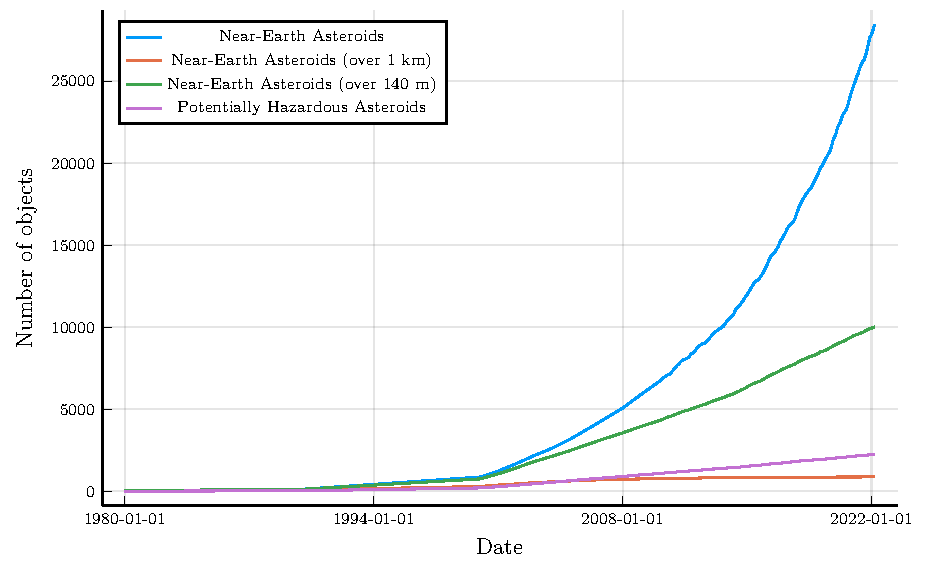
\includegraphics[width=\textwidth]{Figures/Chapter1/jpl_nea_data.pdf}
	\caption{Near-Earth Asteroids cataloged over the years. Today, about 8\% of them are classified as Potentially Hazardous Asteroids (data from \cite{nea_stats_jpl})}
	\label{fig:NEA_nasa}
\end{figure}

\subsection{Techniques for collision avoidance}
\label{ssec:collision_avoidance}


\section{The Asteroid Impact and Deflection Assessment (AIDA)}
\chapter{Methodology \& Model design}
\label{chap:methodology}

\section{Programming Language}
\label{sec:language}

Given the computational nature of the orbit determination problem introduced in \Cref{chap:introduction}, a decision for the appropriate programming language in which the model will be developed has to be made. In today's academic environment, several scientists chose to develop their code in dynamic languages such as MATLAB or Python, which enhance productivity by giving a variety of tools to developers. However, these dynamic programming languages suffer during problems which can be classified as computationally intensive, leading to the use of languages such as C or Fortran when dealing computationally heavy problems \cite{Julia-2017}. 

The problem with the latter languages is that they do not offer the productivity provided by the dynamic languages, which have arguably made the development of scientific code fairly easier, leading to developers having to perform a trade-off for each problem to choose the appropriate language.  This problem is frequently described as the two language problem in literature. A solution which combines both the productivity and performance and thus solves the two language problem is Julia \cite{Julia-2017}. From \Cref{fig:julia_bench}, it can be concluded that code written in Julia will achieve similar benchmark times to C \cite{julia-benchmark}, while also providing the user with high level functions and options to write code in a more productive manner.

\begin{figure}[h]
	\centering
	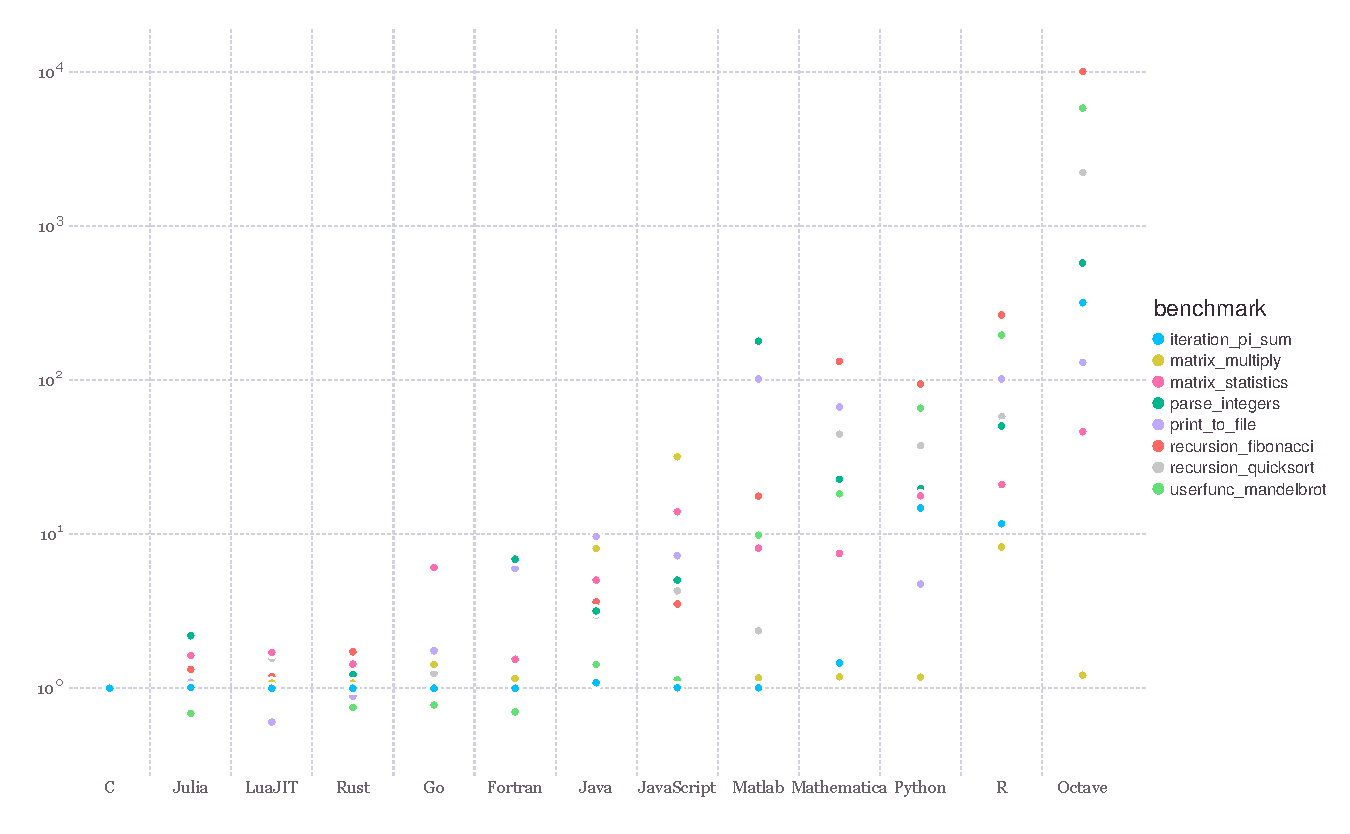
\includegraphics[width=\textwidth]{Figures/Chapter2/julia_benchmarks.pdf}
	\caption{Normalized benchmark time of some problems against the C implementation for different programming languages \cite{julia-benchmark}}
	\label{fig:julia_bench}
\end{figure}

In the context of this thesis, it can be expected that the code developed will be computationally intensive, given the fact that numerical integrators used to perform the propagation of the asteroids for the fitting procedure (which will undoubtedly run several times until a solution is identified), leading to a need for performance. In addition, coordinate transformations, missing objects from the images generated and other pitfalls require a productive way to deal with these problems. Since the two language problem is being faced, the decision has been made early to use Julia as the programming language for the development of this thesis.

\section{Orbital Dynamics}

For the description of the orbit determination problem being faced from the perspective of astrodynamics, we can simplify the problem into two separate problems, namely:

\begin{enumerate}
	\item The orbit followed by the Hera spacecraft during the observation period.
	\item The behavior of the two asteroids Didymos \& Dimorphos.
\end{enumerate}

Once an adequate description for both of these sub-problems has been given, they can then combine them into a single dynamics model using the appropriate reference frames and transformations between them. After this combination is complete, the image generation procedure can be built and different types of errors can be added.  
   
   
\subsection{Hera Spacecraft}

As briefly discussed in %insert chapter reference from Chapter 1
, the Hera spacecraft will follow hyperbolic trajectories. This is based on the legacy from a previous mission to a small body. The Rosetta mission visited the comet 67P/Churyumov-Gerasimenko in 2014. The Rosetta spacecraft implemented hyperbolic trajectories for a variety of reasons described by \citeauthor{rosetta-orbit} \cite{rosetta-orbit}, which include:

\begin{enumerate}
	\item Poor gravity potential estimates to plan an accurate circular or elliptic orbit.
	\item Large approach velocities for circular orbits when compared to orbital velocities.
	\item Lower sensitivity to insertion maneuver errors for hyperbolic trajectories. 
	\item The hyperbolic trajectory arcs can be designed in a manner which ensures that the sun remains behind the spacecraft at all times, providing good observation conditions. 
	\item The cost in terms of $\Delta v$ for the maintenance of the hyperbolic arcs remains fairly small, usually at the order of $\frac{\si{\centi\meter}}{\si{\second}}$.
\end{enumerate}

These problems remain applicable to the Didymos-Dimorphos asteroid system. Based on the expertise from Rosetta, ESA will command Hera to fly trajectories with pericentre velocity larger than the escape velocity, with a safety margin $C$, as defined in \Cref{eq:hera_velocity} \cite{hera-autonomous-ops}.

\begin{equation}
	\label{eq:hera_velocity}
	v_{p e r i}=(1+C) \sqrt{\frac{2 \mu}{r_{p e r i}}} \quad, \quad C>0
\end{equation}

The safety margin ensures that no collision can occur during an arc due to the presence of uncertainties in the gravity field model and is assigned a value of $C=0.4$ for Hera proximity operations \cite{hera-autonomous-ops}.

\subsection{SPICE and SPICE.jl}
\label{sec:spice}

Given all of this information, hyperbolic arcs can be defined at will. However, to ensure consistency with the actual implementation of Hera's orbit, the hyperbolic arcs of Hera will be extracted from SPICE. SPICE provides a portable, multi-discipline mechanism useful in both planning space science observations and defining the position of objects with respect to pre-defined reference frames \cite{SPICE}. SPICE is comprised of different logical elements which also form the acronym SPICE (Spacecraft, Planet, Instrument, Camera matrix and Events) and correspond to different SPICE data products which can then be used by end users for different applications\cite{SPICE}. An overview of the SPICE architecture can be found in \Cref{fig:spice_components}. Most notably, we are interested in the following SPICE kernels:

\begin{itemize}
	\item \textbf{SPK}, which provide position and velocity of spacecraft and different bodies as a function of time.
	\item \textbf{LSK}, which house the leapseconds kernel required for time computations. 
	\item \textbf{IK}, which house information about specific instruments on-board a spacecraft
	\item \textbf{CK}, which provide orientation of a camera instrument ("camera matrix") for specific time intervals.
	\item \textbf{FK}, which offer access to a number of reference frames which can then be used to transform coordinates between reference frames.
\end{itemize}

\begin{figure}[h]
	\centering
	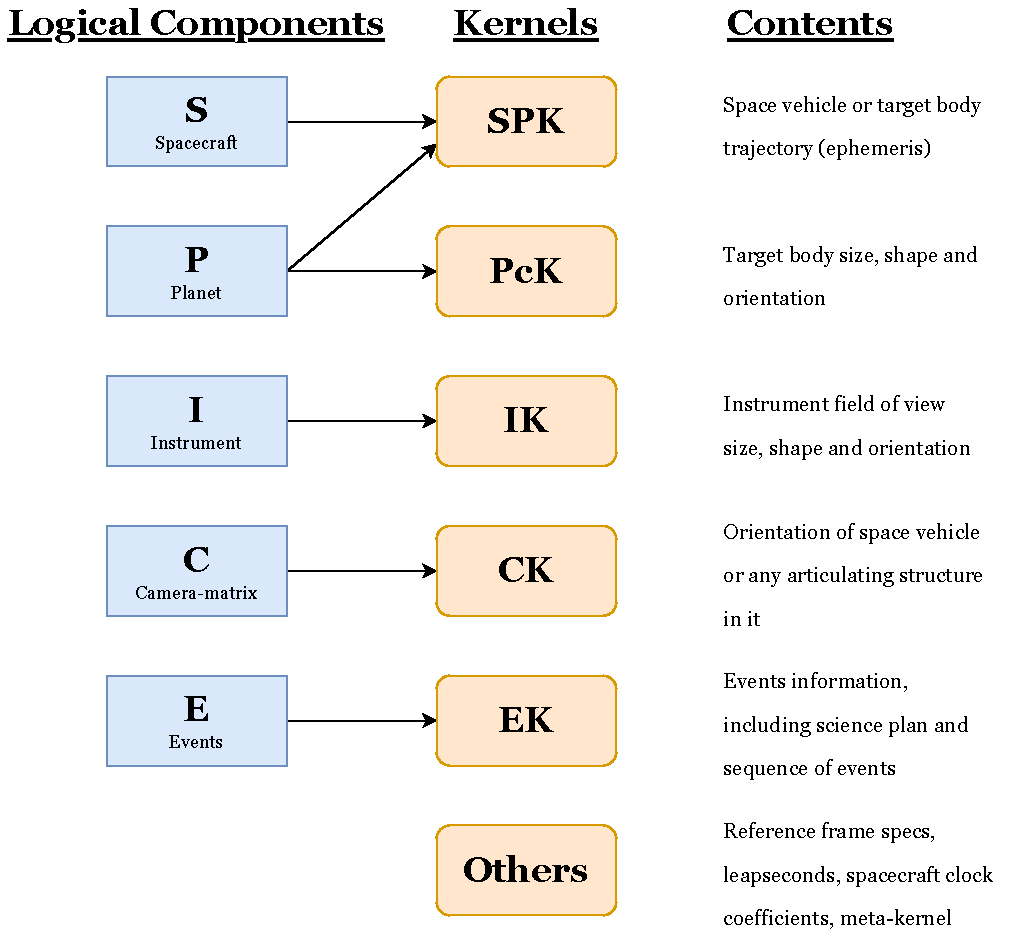
\includegraphics[width=\textwidth]{Figures/Chapter2/spice_components.pdf}
	\caption{Explanation of the SPICE architecture \cite{SPICE}}
	\label{fig:spice_components}
\end{figure}

The European Space Agency has a dedicated department called the ESA SPICE Service, which is located at the European Space Astronomy Center. ESA SPICE Service is responsible for the creation and distribution of SPICE data for a number of ESA missions, including the hera mission which is of interest to us \cite{esa-spice-hera}. The repository is updated every few months with the most up-to-date SPICE data based on revised estimates and/or new observational data. For this thesis, the Hera SPICE Kernel Dataset version 1.1 dated 09/11/2021 is used. To access the SPICE data provided, a dedicated Julia wrapper for the SPICE toolkit has to be used to convert the data to a usable format. This wrapper is SPICE.jl.  

As previously discussed in \Cref{chap:introduction}, the dynamical characterization of the Didymos-Dimorphos binary asteroid system takes place during the first of the six proximity operation phases, namely during the Early Characterization Phase \cite{hera-autonomous-ops}. During this phase, Hera performs hyperbolic arcs with the main objective of capturing images to perform a physical and dynamical characterization of the system \cite{hera-autonomous-ops}. Typical orbits followed by Hera during this phase can be seen in \Cref{fig:hera_extended_orbit}, which has been extracted directly from the SPICE data discussed before. In 

\begin{figure}[h]
	\centering
	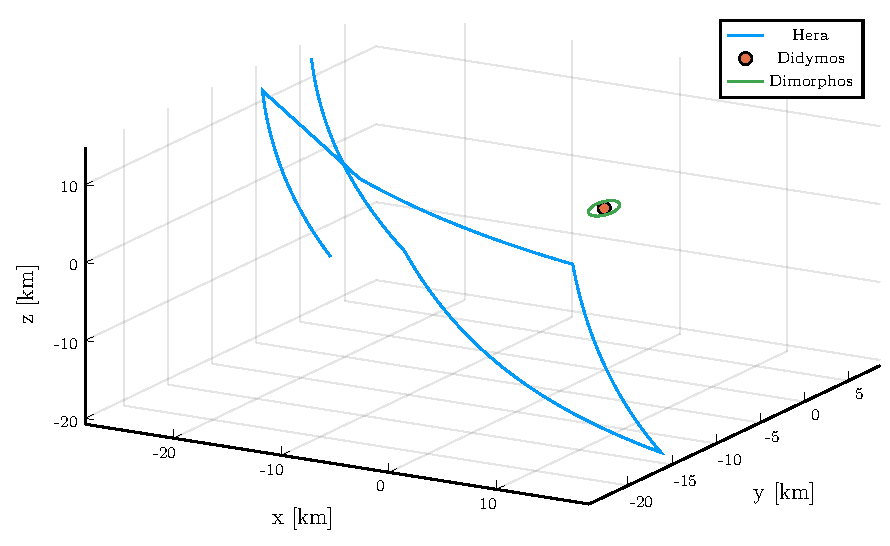
\includegraphics[width=\textwidth]{Figures/Chapter2/ECP_extended_reference_plot.pdf}
	\caption{Five hyperbolic arcs performed by Hera with respect to the system's barycenter over a period of 15 days.}
	\label{fig:hera_extended_orbit}
\end{figure}

For the context of this thesis, a time interval corresponding to 5 hyperbolic arcs has been chosen. The observation time used has been set to achieve this is set to \si{300 \hour}, which is approximately equivalent to 25 orbits of Dimorphos around Didymos. This observation period is equal to \num{12.5} days, providing a reasonable time frame for the acquisition of pictures. At the worst case scenario, assuming that Hera has to acquire \num{1000} photos of the two asteroids, approximately \num{4} photos per hour have to be taken, providing enough time per hour for other operations including orbital maintenance. One also has to note that due to high pointing errors especially towards the end of a hyperbolic arc \cite{hera-adcs}, pointing errors would fluctuate even more for longer observation periods. 

\begin{figure}[h]
	\centering
	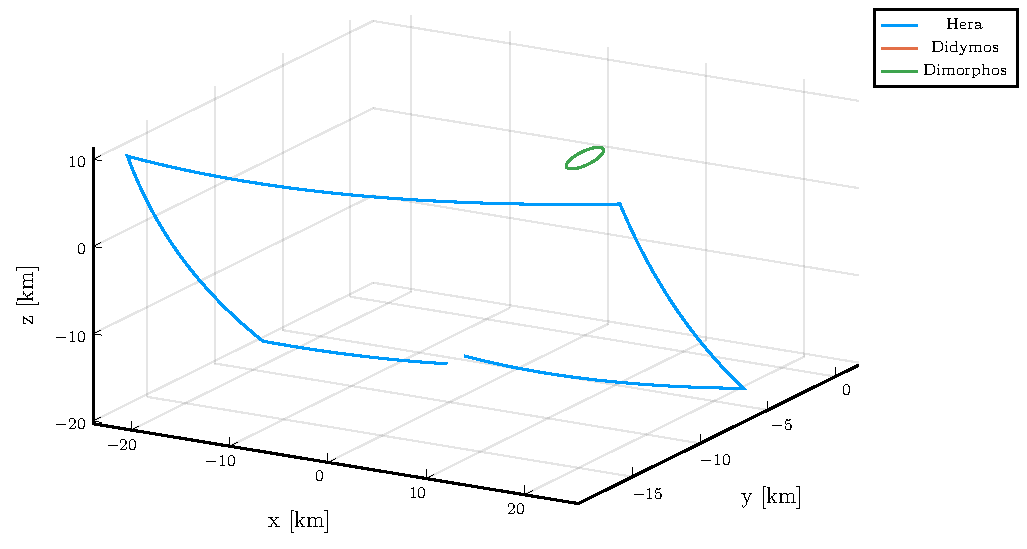
\includegraphics[width=\textwidth]{Figures/Chapter2/ECP_thesis_orbit_plot.pdf}
	\caption{The hyperbolic arcs which Hera orbits on during the \si{300\hour} observation period chosen for this thesis.}
	\label{fig:hera_thesis_orbit}
\end{figure}

Finally, the observation period selected includes four transitions between hyperbolic arcs, which correspond to the worst observational conditions, where the pointing error gets maximized \cite{hera-adcs}. The corresponding orbit of Hera for the selected time interval during the Early Characterization Phase with respect to the system's barycenter can be seen in \Cref{fig:hera_thesis_orbit}. 

\subsection{Didymos-Dimorphos dynamics}

In \Cref{sec:spice}, the orbits of all bodies were extracted with respect to the barycenter of the Didymos-Dimorphos system. While the orbit of the Hera spacecraft will be extracted and used directly from SPICE, the orbits of the two asteroids will be extracted from a self-developed Runge-Kutta 4 integrator. This will enable testing of several types of orbits and orbital parameters, which are not limited by the one reference case included in the data provided by the ESA SPICE Service. The properties of the system and the integrator will be discussed now. 

Since Hera's orbit is predefined from SPICE and does not have to be calculated, the two body problem can be used for the two asteroids. The gravitational force between two bodies is given by:

\begin{equation}
	\overrightarrow{F_{i}}=G \frac{m_{i} m_{j}}{r_{i j}^{3}} \overrightarrow{r_{i j}}
\end{equation}

While the equation of motion for each body is given by:

\begin{equation}
	\ddot{\overrightarrow{R}_{i}}=G \frac{m_{j}}{r_{i j}^{3}} \overrightarrow{r_{i j}}
\end{equation}

The equation of relative motion will thus be given by:

\begin{equation}
	\ddot{\overrightarrow{r}} = -G\left(m_{1}+m_{2}\right) \frac{\overrightarrow{r}}{r^{3}}
\end{equation}

Being a small asteroid body, Didymos does not have atmosphere which can cause a perturbation to the motion of Dimorphos due to atmospheric drag. However, the non-spherical shape of the asteroid will cause a perturbation in the gravitational potential. While one of the main goals of the DART mission is to obtain a better understanding of the gravity environment of the binary asteroid system \cite{dart-requirements}, only perturbations caused by $J_2$ will be considered in this thesis. This perturbation will cause the variation of orbital elements throughout the period of the orbit and will allow us to model complex situations by working with osculating elements. Considering the effect of $J_{2}$, the equation of relative motion which we will use will be:

\begin{equation}
	\ddot{\overrightarrow{r}} = -G\left(m_{Didymos}+m_{Dimorphos}\right) \frac{\overrightarrow{r}}{r^{3}} + \overrightarrow{a_{J_2}}
\end{equation}

The acceleration caused by $J_{2}$ can be written in cartesian form as \cite{vallado}:

\begin{equation}
	a_{i}=-\frac{3 J_{2} \mu R_{didymos}^{2} r_{i}}{2 r^{5}}\left(1-\frac{5 r_{k}^{2}}{r^{2}}\right)
\end{equation}

\begin{equation}
	a_{j}=-\frac{3 J_{2} \mu R_{didymos}^{2} r_{j}}{2 r^{5}}\left(1-\frac{5 r_{k}^{2}}{r^{2}}\right)
\end{equation}

\begin{equation}
	a_{k}=-\frac{3 J_{2} \mu R_{didymos}^{2} r_{k}}{2 r^{5}}\left(3-\frac{5 r_{k}^{2}}{r^{2}}\right)
\end{equation}

where $\mu= G\left(M_{didymos} + M_{dimorphos} \right)$ and $i,\ j$ and $k$ correspond to $x,\ y$ and $z$ coordinates. The final form of the equations of motion for each cartesian coordinate to be integrated are:

\begin{equation}
	\label{eq:motionx}
	\ddot{x} = -\frac{\mu x}{r^{3}} -\frac{3 J_{2} \mu R_{didymos}^{2} r_{i}}{2 r^{5}}\left(1-\frac{5 r_{k}^{2}}{r^{2}}\right)
\end{equation}

\begin{equation}
	\label{eq:motiony}
	\ddot{y} = -\frac{\mu y}{r^{3}} -\frac{3 J_{2} \mu R_{didymos}^{2} r_{j}}{2 r^{5}}\left(1-\frac{5 r_{k}^{2}}{r^{2}}\right)
\end{equation}

\begin{equation}
	\label{eq:motionz}
	\ddot{z} = -\frac{\mu z}{r^{3}} -\frac{3 J_{2} \mu R_{didymos}^{2} r_{k}}{2 r^{5}}\left(3-\frac{5 r_{k}^{2}}{r^{2}}\right)
\end{equation}

\Cref{eq:motionx,eq:motiony,eq:motionz} form a system of differential equations which have to be integrated. To integrate the system, a Runge-Kutta method will be used, which achieves the accuracy of a Taylor series approach without requiring the calculation of higher derivatives \cite{chapra}. A fourth order Runge-Kutta method will be used here (RK4), where the solution is given by the iterative form of:

\begin{equation}
	y_{i+1}=y{i}+\frac{1}{6}\left( k_{1} + 2k_{2} + 2k_{3} + k_{4}\right)
\end{equation}

The $k$ constants are computed using:

\begin{equation}
\label{eq:rk4-constants}
\begin{aligned}
		k_{1} &= f(x_{i},y_{i})\\
		k_{2} &= f(x_{i}+\frac{h}{2},y_{i}+\frac{k_{1}h}{2})\\
		k_{3} &= f\left( x_{i}+\frac{h}{2},y_{i}+\frac{k_{2}h}{2} \right)\\
		k_{4} &= f(x_{i}+h,y_{i}+k_{3}h)
\end{aligned}
\end{equation}

In \Cref{eq:rk4-constants}, $h$ refers to the step size used for the integration, which in this case is the time step used. We will use a time step of $dt=60$ \si{\second}. To ensure that the integrator works properly, it has been validated against the PKEPLER routine \cite{vallado}. The validation procedure has showed that the cartesian positions and velocities obtained using the RK4 integrator used here fully coincides with the cartesian positions and velocities obtained using the PKEPLER routine. The full validation procedure and the results obtained can be found in \Cref{appendix:rk4-validation}.

\subsection{Didymos $J_{2}$}

To compute the $J_{2}$ constant of Didymos, the moments of inertia of the asteroid are used. Let's derive the $J_{2}$ constant now. The expressions of inertial integrals for a rigid body will be used \cite{scheeres}, which provide a relationship for the moment of inertia and the zonal gravitational coefficients, namely:

\begin{equation}
	\label{eq:inertia-first}
	I_{xx} - I_{yy} = -4Mr_{o}^{2}C_{22}
\end{equation}

and:

\begin{equation}
	\label{eq:inertia-second}
	I_{yy} - I_{zz} = Mr_{o}^{2} (C_{20} + 2C_{22})
\end{equation}

Combining \cref{eq:inertia-first} and \cref{eq:inertia-second} yields:

\begin{equation}
	\label{eq:inertia-c20}
	-C_{20} = \frac{2I_{zz}-I_{yy}-I_{xx}}{2Mr_{o}^{2}}
\end{equation}

taking into consideration the fact that $J_{2}=-C_{20}$, the final expression for $J_{2}$ is obtained to be:

\begin{equation}
	\label{eq:inertia-j2}
	J_{2} = \frac{2I_{zz}-I_{yy}-I_{xx}}{2Mr_{o}^{2}}
\end{equation}

Let's assume Didymos to be a triaxial ellipsoid and obtain a mean radius for the body. Assuming $a=0.416194$ \si{\kilo\meter} and $b=0.418765$ \si{\kilo\meter}, a radius value is obtained to be:

\begin{equation}
	R=\frac{a+b}{2}=0.4174795\ km
\end{equation}

For Didymos, a mass of $M_{Didymos}=5.32\times10^{11}$ \si{\kilogram} will be used. The moments of inertia are computed to be such that there is an alignment of results with the results computed by the General Use Binary Asteroid Simulator (GUBAS) \cite{gubas}, and are presented in \Cref{tab:inertia-didymos}. Combining all of these values together in \Cref{eq:inertia-j2}, a final value of $J_{2}$ is obtained to be:

\begin{equation}
	\label{eq:final-j2}
	J_{2} = 0.012503167534491537
\end{equation}

this value will be used in the RK4 propagator to introduce the perturbation in all instances from now on.

\begin{table}[h]
	\centering
	\caption{Moments of Inertia for Didymos}
	\begin{tabular}{c c}
		\toprule
		\textbf{Moments of Inertia} & \textbf{Value [\si{\kilogram \kilo\meter\squared}]} \\
		\midrule
		\textbf{$I_{xx}$}        & 31436.196699045453 \\
		\textbf{$I_{yy}$}       & 32009.61802392827   \\      
		\textbf{$I_{zz}$}       & 32882.223794965415  \\
		\bottomrule
	\end{tabular}
	\label{tab:inertia-didymos}
\end{table}
%\chapter{Methodology \& Model design}
\label{chap:methodology}

\section{Programming Language}
\label{sec:language}

Given the computational nature of the orbit determination problem introduced in \Cref{chap:introduction}, a decision for the appropriate programming language in which the model will be developed has to be made. In today's academic environment, several scientists chose to develop their code in dynamic languages such as MATLAB or Python, which enhance productivity by giving a variety of tools to developers. However, these dynamic programming languages suffer during problems which can be classified as computationally intensive, leading to the use of languages such as C or Fortran when dealing computationally heavy problems \cite{Julia-2017}. 

The problem with the latter languages is that they do not offer the productivity provided by the dynamic languages, which have arguably made the development of scientific code fairly easier, leading to developers having to perform a trade-off for each problem to choose the appropriate language.  This problem is frequently described as the two language problem in literature. A solution which combines both the productivity and performance and thus solves the two language problem is Julia \cite{Julia-2017}. From \Cref{fig:julia_bench}, it can be concluded that code written in Julia will achieve similar benchmark times to C \cite{julia-benchmark}, while also providing the user with high level functions and options to write code in a more productive manner.

\begin{figure}[h]
	\centering
	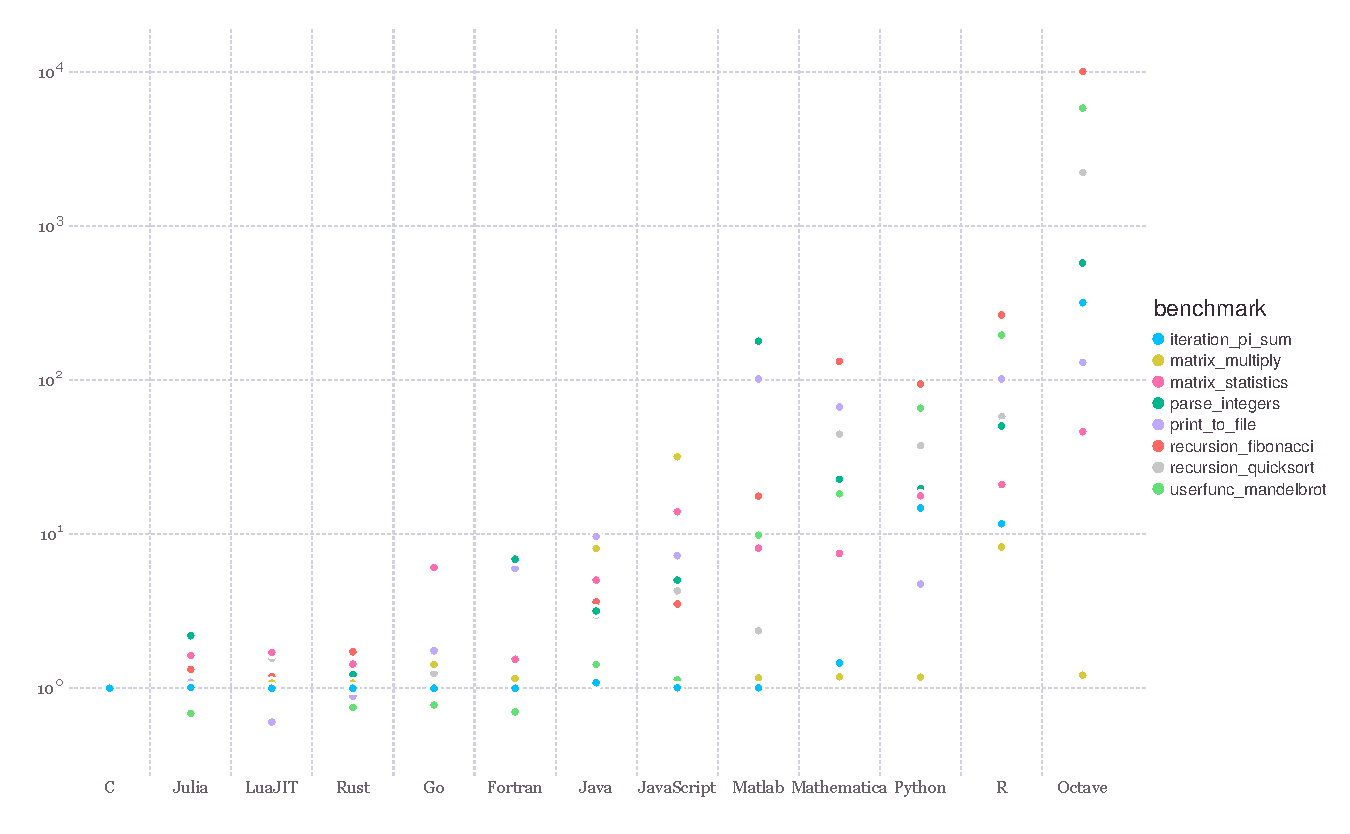
\includegraphics[width=\textwidth]{Figures/Chapter2/julia_benchmarks.pdf}
	\caption{Normalized benchmark time of some problems against the C implementation for different programming languages \cite{julia-benchmark}}
	\label{fig:julia_bench}
\end{figure}

In the context of this thesis, it can be expected that the code developed will be computationally intensive, given the fact that numerical integrators used to perform the propagation of the asteroids for the fitting procedure (which will undoubtedly run several times until a solution is identified), leading to a need for performance. In addition, coordinate transformations, missing objects from the images generated and other pitfalls require a productive way to deal with these problems. Since the two language problem is being faced, the decision has been made early to use Julia as the programming language for the development of this thesis.

\section{Orbital Dynamics}

For the description of the orbit determination problem being faced from the perspective of astrodynamics, we can simplify the problem into two separate problems, namely:

\begin{enumerate}
	\item The orbit followed by the Hera spacecraft during the observation period.
	\item The behavior of the two asteroids Didymos \& Dimorphos.
\end{enumerate}

Once an adequate description for both of these sub-problems has been given, they can then combine them into a single dynamics model using the appropriate reference frames and transformations between them. After this combination is complete, the image generation procedure can be built and different types of errors can be added.  
   
   
\subsection{Hera Spacecraft}

As briefly discussed in %insert chapter reference from Chapter 1
, the Hera spacecraft will follow hyperbolic trajectories. This is based on the legacy from a previous mission to a small body. The Rosetta mission visited the comet 67P/Churyumov-Gerasimenko in 2014. The Rosetta spacecraft implemented hyperbolic trajectories for a variety of reasons described by \citeauthor{rosetta-orbit} \cite{rosetta-orbit}, which include:

\begin{enumerate}
	\item Poor gravity potential estimates to plan an accurate circular or elliptic orbit.
	\item Large approach velocities for circular orbits when compared to orbital velocities.
	\item Lower sensitivity to insertion maneuver errors for hyperbolic trajectories. 
	\item The hyperbolic trajectory arcs can be designed in a manner which ensures that the sun remains behind the spacecraft at all times, providing good observation conditions. 
	\item The cost in terms of $\Delta v$ for the maintenance of the hyperbolic arcs remains fairly small, usually at the order of $\frac{\si{\centi\meter}}{\si{\second}}$.
\end{enumerate}

These problems remain applicable to the Didymos-Dimorphos asteroid system. Based on the expertise from Rosetta, ESA will command Hera to fly trajectories with pericentre velocity larger than the escape velocity, with a safety margin $C$, as defined in \Cref{eq:hera_velocity} \cite{hera-autonomous-ops}.

\begin{equation}
	\label{eq:hera_velocity}
	v_{p e r i}=(1+C) \sqrt{\frac{2 \mu}{r_{p e r i}}} \quad, \quad C>0
\end{equation}

The safety margin ensures that no collision can occur during an arc due to the presence of uncertainties in the gravity field model and is assigned a value of $C=0.4$ for Hera proximity operations \cite{hera-autonomous-ops}.

\subsection{SPICE and SPICE.jl}
\label{sec:spice}

Given all of this information, hyperbolic arcs can be defined at will. However, to ensure consistency with the actual implementation of Hera's orbit, the hyperbolic arcs of Hera will be extracted from SPICE. SPICE provides a portable, multi-discipline mechanism useful in both planning space science observations and defining the position of objects with respect to pre-defined reference frames \cite{SPICE}. SPICE is comprised of different logical elements which also form the acronym SPICE (Spacecraft, Planet, Instrument, Camera matrix and Events) and correspond to different SPICE data products which can then be used by end users for different applications\cite{SPICE}. An overview of the SPICE architecture can be found in \Cref{fig:spice_components}. Most notably, we are interested in the following SPICE kernels:

\begin{itemize}
	\item \textbf{SPK}, which provide position and velocity of spacecraft and different bodies as a function of time.
	\item \textbf{LSK}, which house the leapseconds kernel required for time computations. 
	\item \textbf{IK}, which house information about specific instruments on-board a spacecraft
	\item \textbf{CK}, which provide orientation of a camera instrument ("camera matrix") for specific time intervals.
	\item \textbf{FK}, which offer access to a number of reference frames which can then be used to transform coordinates between reference frames.
\end{itemize}

\begin{figure}[h]
	\centering
	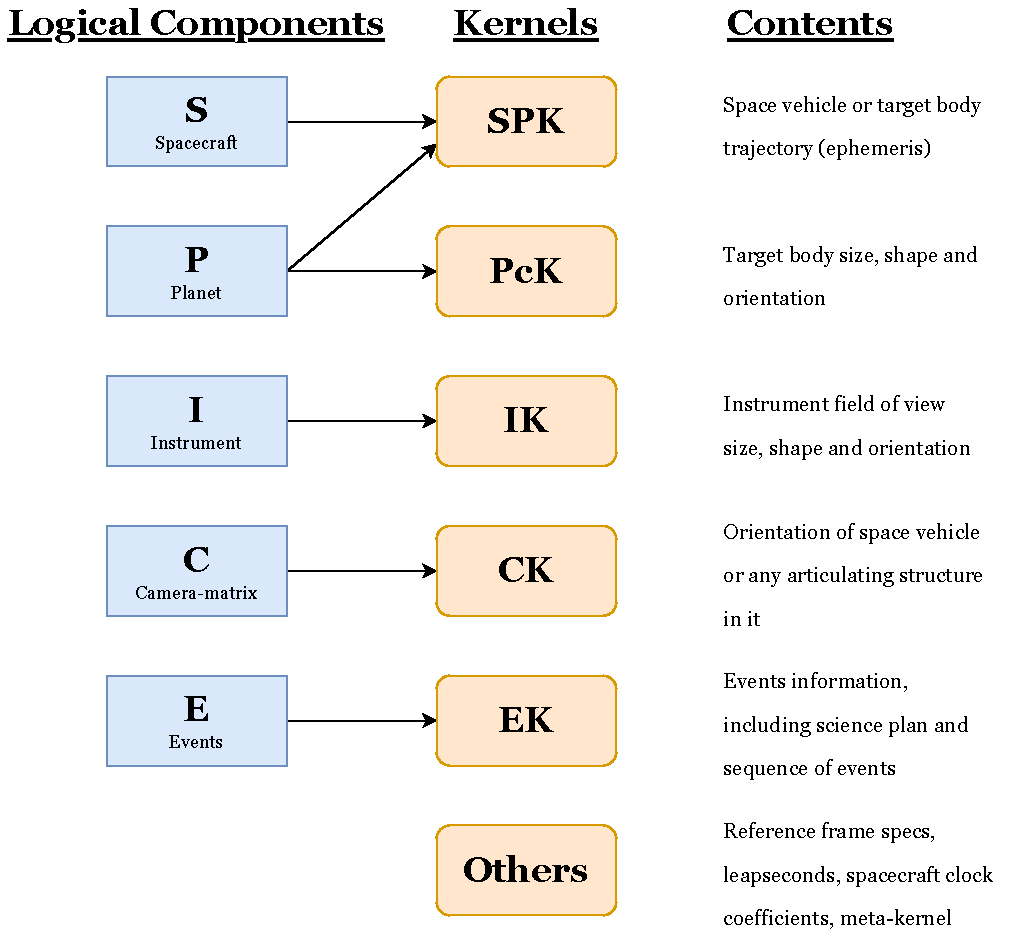
\includegraphics[width=\textwidth]{Figures/Chapter2/spice_components.pdf}
	\caption{Explanation of the SPICE architecture \cite{SPICE}}
	\label{fig:spice_components}
\end{figure}

The European Space Agency has a dedicated department called the ESA SPICE Service, which is located at the European Space Astronomy Center. ESA SPICE Service is responsible for the creation and distribution of SPICE data for a number of ESA missions, including the hera mission which is of interest to us \cite{esa-spice-hera}. The repository is updated every few months with the most up-to-date SPICE data based on revised estimates and/or new observational data. For this thesis, the Hera SPICE Kernel Dataset version 1.1 dated 09/11/2021 is used. To access the SPICE data provided, a dedicated Julia wrapper for the SPICE toolkit has to be used to convert the data to a usable format. This wrapper is SPICE.jl.  

As previously discussed in \Cref{chap:introduction}, the dynamical characterization of the Didymos-Dimorphos binary asteroid system takes place during the first of the six proximity operation phases, namely during the Early Characterization Phase \cite{hera-autonomous-ops}. During this phase, Hera performs hyperbolic arcs with the main objective of capturing images to perform a physical and dynamical characterization of the system \cite{hera-autonomous-ops}. Typical orbits followed by Hera during this phase can be seen in \Cref{fig:hera_extended_orbit}, which has been extracted directly from the SPICE data discussed before. In 

\begin{figure}[h]
	\centering
	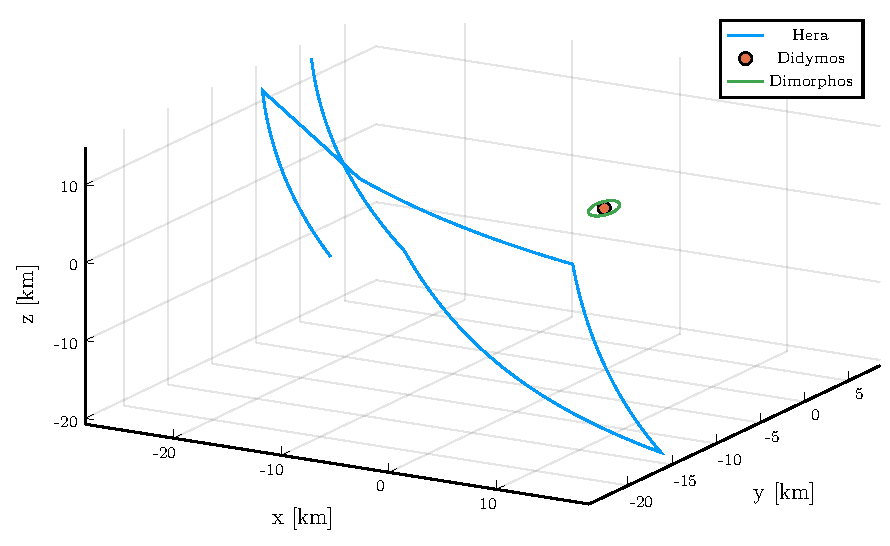
\includegraphics[width=\textwidth]{Figures/Chapter2/ECP_extended_reference_plot.pdf}
	\caption{Five hyperbolic arcs performed by Hera with respect to the system's barycenter over a period of 15 days.}
	\label{fig:hera_extended_orbit}
\end{figure}

For the context of this thesis, a time interval corresponding to 5 hyperbolic arcs has been chosen. The observation time used has been set to achieve this is set to \si{300 \hour}, which is approximately equivalent to 25 orbits of Dimorphos around Didymos. This observation period is equal to \num{12.5} days, providing a reasonable time frame for the acquisition of pictures. At the worst case scenario, assuming that Hera has to acquire \num{1000} photos of the two asteroids, approximately \num{4} photos per hour have to be taken, providing enough time per hour for other operations including orbital maintenance. One also has to note that due to high pointing errors especially towards the end of a hyperbolic arc \cite{hera-adcs}, pointing errors would fluctuate even more for longer observation periods. 

\begin{figure}[h]
	\centering
	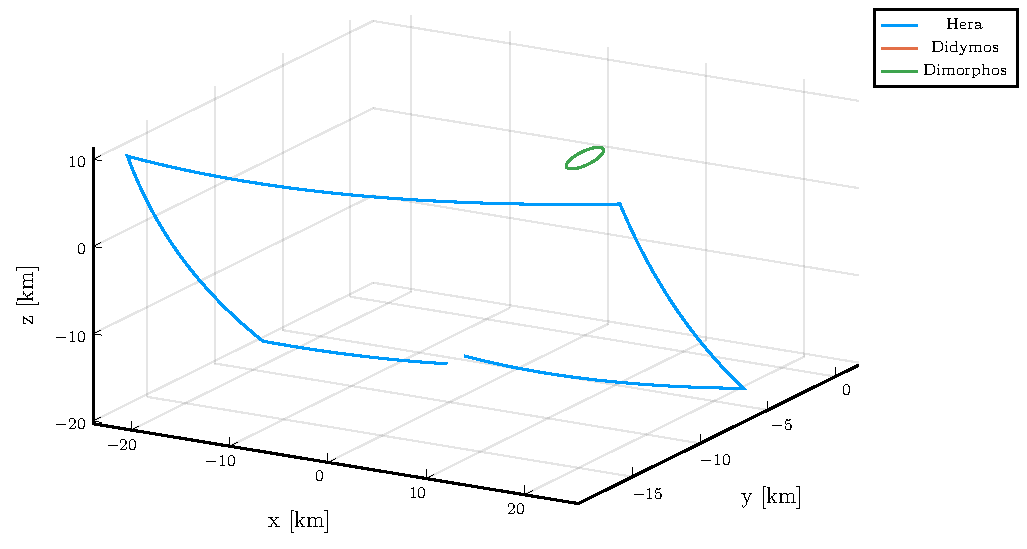
\includegraphics[width=\textwidth]{Figures/Chapter2/ECP_thesis_orbit_plot.pdf}
	\caption{The hyperbolic arcs which Hera orbits on during the \si{300\hour} observation period chosen for this thesis.}
	\label{fig:hera_thesis_orbit}
\end{figure}

Finally, the observation period selected includes four transitions between hyperbolic arcs, which correspond to the worst observational conditions, where the pointing error gets maximized \cite{hera-adcs}. The corresponding orbit of Hera for the selected time interval during the Early Characterization Phase with respect to the system's barycenter can be seen in \Cref{fig:hera_thesis_orbit}. 

\subsection{Didymos-Dimorphos dynamics}

In \Cref{sec:spice}, the orbits of all bodies were extracted with respect to the barycenter of the Didymos-Dimorphos system. While the orbit of the Hera spacecraft will be extracted and used directly from SPICE, the orbits of the two asteroids will be extracted from a self-developed Runge-Kutta 4 integrator. This will enable testing of several types of orbits and orbital parameters, which are not limited by the one reference case included in the data provided by the ESA SPICE Service. The properties of the system and the integrator will be discussed now. 

Since Hera's orbit is predefined from SPICE and does not have to be calculated, the two body problem can be used for the two asteroids. The gravitational force between two bodies is given by:

\begin{equation}
	\overrightarrow{F_{i}}=G \frac{m_{i} m_{j}}{r_{i j}^{3}} \overrightarrow{r_{i j}}
\end{equation}

While the equation of motion for each body is given by:

\begin{equation}
	\ddot{\overrightarrow{R}_{i}}=G \frac{m_{j}}{r_{i j}^{3}} \overrightarrow{r_{i j}}
\end{equation}

The equation of relative motion will thus be given by:

\begin{equation}
	\ddot{\overrightarrow{r}} = -G\left(m_{1}+m_{2}\right) \frac{\overrightarrow{r}}{r^{3}}
\end{equation}

Being a small asteroid body, Didymos does not have atmosphere which can cause a perturbation to the motion of Dimorphos due to atmospheric drag. However, the non-spherical shape of the asteroid will cause a perturbation in the gravitational potential. While one of the main goals of the DART mission is to obtain a better understanding of the gravity environment of the binary asteroid system \cite{dart-requirements}, only perturbations caused by $J_2$ will be considered in this thesis. This perturbation will cause the variation of orbital elements throughout the period of the orbit and will allow us to model complex situations by working with osculating elements. Considering the effect of $J_{2}$, the equation of relative motion which we will use will be:

\begin{equation}
	\ddot{\overrightarrow{r}} = -G\left(m_{Didymos}+m_{Dimorphos}\right) \frac{\overrightarrow{r}}{r^{3}} + \overrightarrow{a_{J_2}}
\end{equation}

The acceleration caused by $J_{2}$ can be written in cartesian form as \cite{vallado}:

\begin{equation}
	a_{i}=-\frac{3 J_{2} \mu R_{didymos}^{2} r_{i}}{2 r^{5}}\left(1-\frac{5 r_{k}^{2}}{r^{2}}\right)
\end{equation}

\begin{equation}
	a_{j}=-\frac{3 J_{2} \mu R_{didymos}^{2} r_{j}}{2 r^{5}}\left(1-\frac{5 r_{k}^{2}}{r^{2}}\right)
\end{equation}

\begin{equation}
	a_{k}=-\frac{3 J_{2} \mu R_{didymos}^{2} r_{k}}{2 r^{5}}\left(3-\frac{5 r_{k}^{2}}{r^{2}}\right)
\end{equation}

where $\mu= G\left(M_{didymos} + M_{dimorphos} \right)$ and $i,\ j$ and $k$ correspond to $x,\ y$ and $z$ coordinates. The final form of the equations of motion for each cartesian coordinate to be integrated are:

\begin{equation}
	\label{eq:motionx}
	\ddot{x} = -\frac{\mu x}{r^{3}} -\frac{3 J_{2} \mu R_{didymos}^{2} r_{i}}{2 r^{5}}\left(1-\frac{5 r_{k}^{2}}{r^{2}}\right)
\end{equation}

\begin{equation}
	\label{eq:motiony}
	\ddot{y} = -\frac{\mu y}{r^{3}} -\frac{3 J_{2} \mu R_{didymos}^{2} r_{j}}{2 r^{5}}\left(1-\frac{5 r_{k}^{2}}{r^{2}}\right)
\end{equation}

\begin{equation}
	\label{eq:motionz}
	\ddot{z} = -\frac{\mu z}{r^{3}} -\frac{3 J_{2} \mu R_{didymos}^{2} r_{k}}{2 r^{5}}\left(3-\frac{5 r_{k}^{2}}{r^{2}}\right)
\end{equation}

\Cref{eq:motionx,eq:motiony,eq:motionz} form a system of differential equations which have to be integrated. To integrate the system, a Runge-Kutta method will be used, which achieves the accuracy of a Taylor series approach without requiring the calculation of higher derivatives \cite{chapra}. A fourth order Runge-Kutta method will be used here (RK4), where the solution is given by the iterative form of:

\begin{equation}
	y_{i+1}=y{i}+\frac{1}{6}\left( k_{1} + 2k_{2} + 2k_{3} + k_{4}\right)
\end{equation}

The $k$ constants are computed using:

\begin{equation}
\label{eq:rk4-constants}
\begin{aligned}
		k_{1} &= f(x_{i},y_{i})\\
		k_{2} &= f(x_{i}+\frac{h}{2},y_{i}+\frac{k_{1}h}{2})\\
		k_{3} &= f\left( x_{i}+\frac{h}{2},y_{i}+\frac{k_{2}h}{2} \right)\\
		k_{4} &= f(x_{i}+h,y_{i}+k_{3}h)
\end{aligned}
\end{equation}

In \Cref{eq:rk4-constants}, $h$ refers to the step size used for the integration, which in this case is the time step used. We will use a time step of $dt=60$ \si{\second}. To ensure that the integrator works properly, it has been validated against the PKEPLER routine \cite{vallado}. The validation procedure has showed that the cartesian positions and velocities obtained using the RK4 integrator used here fully coincides with the cartesian positions and velocities obtained using the PKEPLER routine. The full validation procedure and the results obtained can be found in \Cref{appendix:rk4-validation}.

\subsection{Didymos $J_{2}$}

To compute the $J_{2}$ constant of Didymos, the moments of inertia of the asteroid are used. Let's derive the $J_{2}$ constant now. The expressions of inertial integrals for a rigid body will be used \cite{scheeres}, which provide a relationship for the moment of inertia and the zonal gravitational coefficients, namely:

\begin{equation}
	\label{eq:inertia-first}
	I_{xx} - I_{yy} = -4Mr_{o}^{2}C_{22}
\end{equation}

and:

\begin{equation}
	\label{eq:inertia-second}
	I_{yy} - I_{zz} = Mr_{o}^{2} (C_{20} + 2C_{22})
\end{equation}

Combining \cref{eq:inertia-first} and \cref{eq:inertia-second} yields:

\begin{equation}
	\label{eq:inertia-c20}
	-C_{20} = \frac{2I_{zz}-I_{yy}-I_{xx}}{2Mr_{o}^{2}}
\end{equation}

taking into consideration the fact that $J_{2}=-C_{20}$, the final expression for $J_{2}$ is obtained to be:

\begin{equation}
	\label{eq:inertia-j2}
	J_{2} = \frac{2I_{zz}-I_{yy}-I_{xx}}{2Mr_{o}^{2}}
\end{equation}

Let's assume Didymos to be a triaxial ellipsoid and obtain a mean radius for the body. Assuming $a=0.416194$ \si{\kilo\meter} and $b=0.418765$ \si{\kilo\meter}, a radius value is obtained to be:

\begin{equation}
	R=\frac{a+b}{2}=0.4174795\ km
\end{equation}

For Didymos, a mass of $M_{Didymos}=5.32\times10^{11}$ \si{\kilogram} will be used. The moments of inertia are computed to be such that there is an alignment of results with the results computed by the General Use Binary Asteroid Simulator (GUBAS) \cite{gubas}, and are presented in \Cref{tab:inertia-didymos}. Combining all of these values together in \Cref{eq:inertia-j2}, a final value of $J_{2}$ is obtained to be:

\begin{equation}
	\label{eq:final-j2}
	J_{2} = 0.012503167534491537
\end{equation}

this value will be used in the RK4 propagator to introduce the perturbation in all instances from now on.

\begin{table}[h]
	\centering
	\caption{Moments of Inertia for Didymos}
	\begin{tabular}{c c}
		\toprule
		\textbf{Moments of Inertia} & \textbf{Value [\si{\kilogram \kilo\meter\squared}]} \\
		\midrule
		\textbf{$I_{xx}$}        & 31436.196699045453 \\
		\textbf{$I_{yy}$}       & 32009.61802392827   \\      
		\textbf{$I_{zz}$}       & 32882.223794965415  \\
		\bottomrule
	\end{tabular}
	\label{tab:inertia-didymos}
\end{table} 
%\include{Chapters/Chapter4} 
%\include{Chapters/Chapter5} 

%----------------------------------------------------------------------------------------
%	THESIS CONTENT - APPENDICES
%----------------------------------------------------------------------------------------

\appendix % Cue to tell LaTeX that the following "chapters" are Appendices

% Include the appendices of the thesis as separate files from the Appendices folder
% Uncomment the lines as you write the Appendices

\include{Appendices/AppendixSourceCode}
%\include{Appendices/AppendixDecay}
%\include{Appendices/AppendixMissionAnalysis}
%\include{Appendices/AppendixMathematica}
%\include{Appendices/AppendixUnstabelSolution}
%\include{Appendices/AppendixStableSolution}

%----------------------------------------------------------------------------------------
%	BIBLIOGRAPHY
%----------------------------------------------------------------------------------------

\printbibliography[heading=bibintoc]

%----------------------------------------------------------------------------------------

\end{document}  
